\documentclass[border=10pt]{standalone}
\usepackage[svgnames]{xcolor}
\usepackage{amsmath}
\usepackage{pgfplots}
\pgfplotsset{compat=newest}
\usepackage[sfdefault]{FiraSans}
\usepackage{FiraMono}
\renewcommand*\familydefault{\sfdefault}
\begin{document}
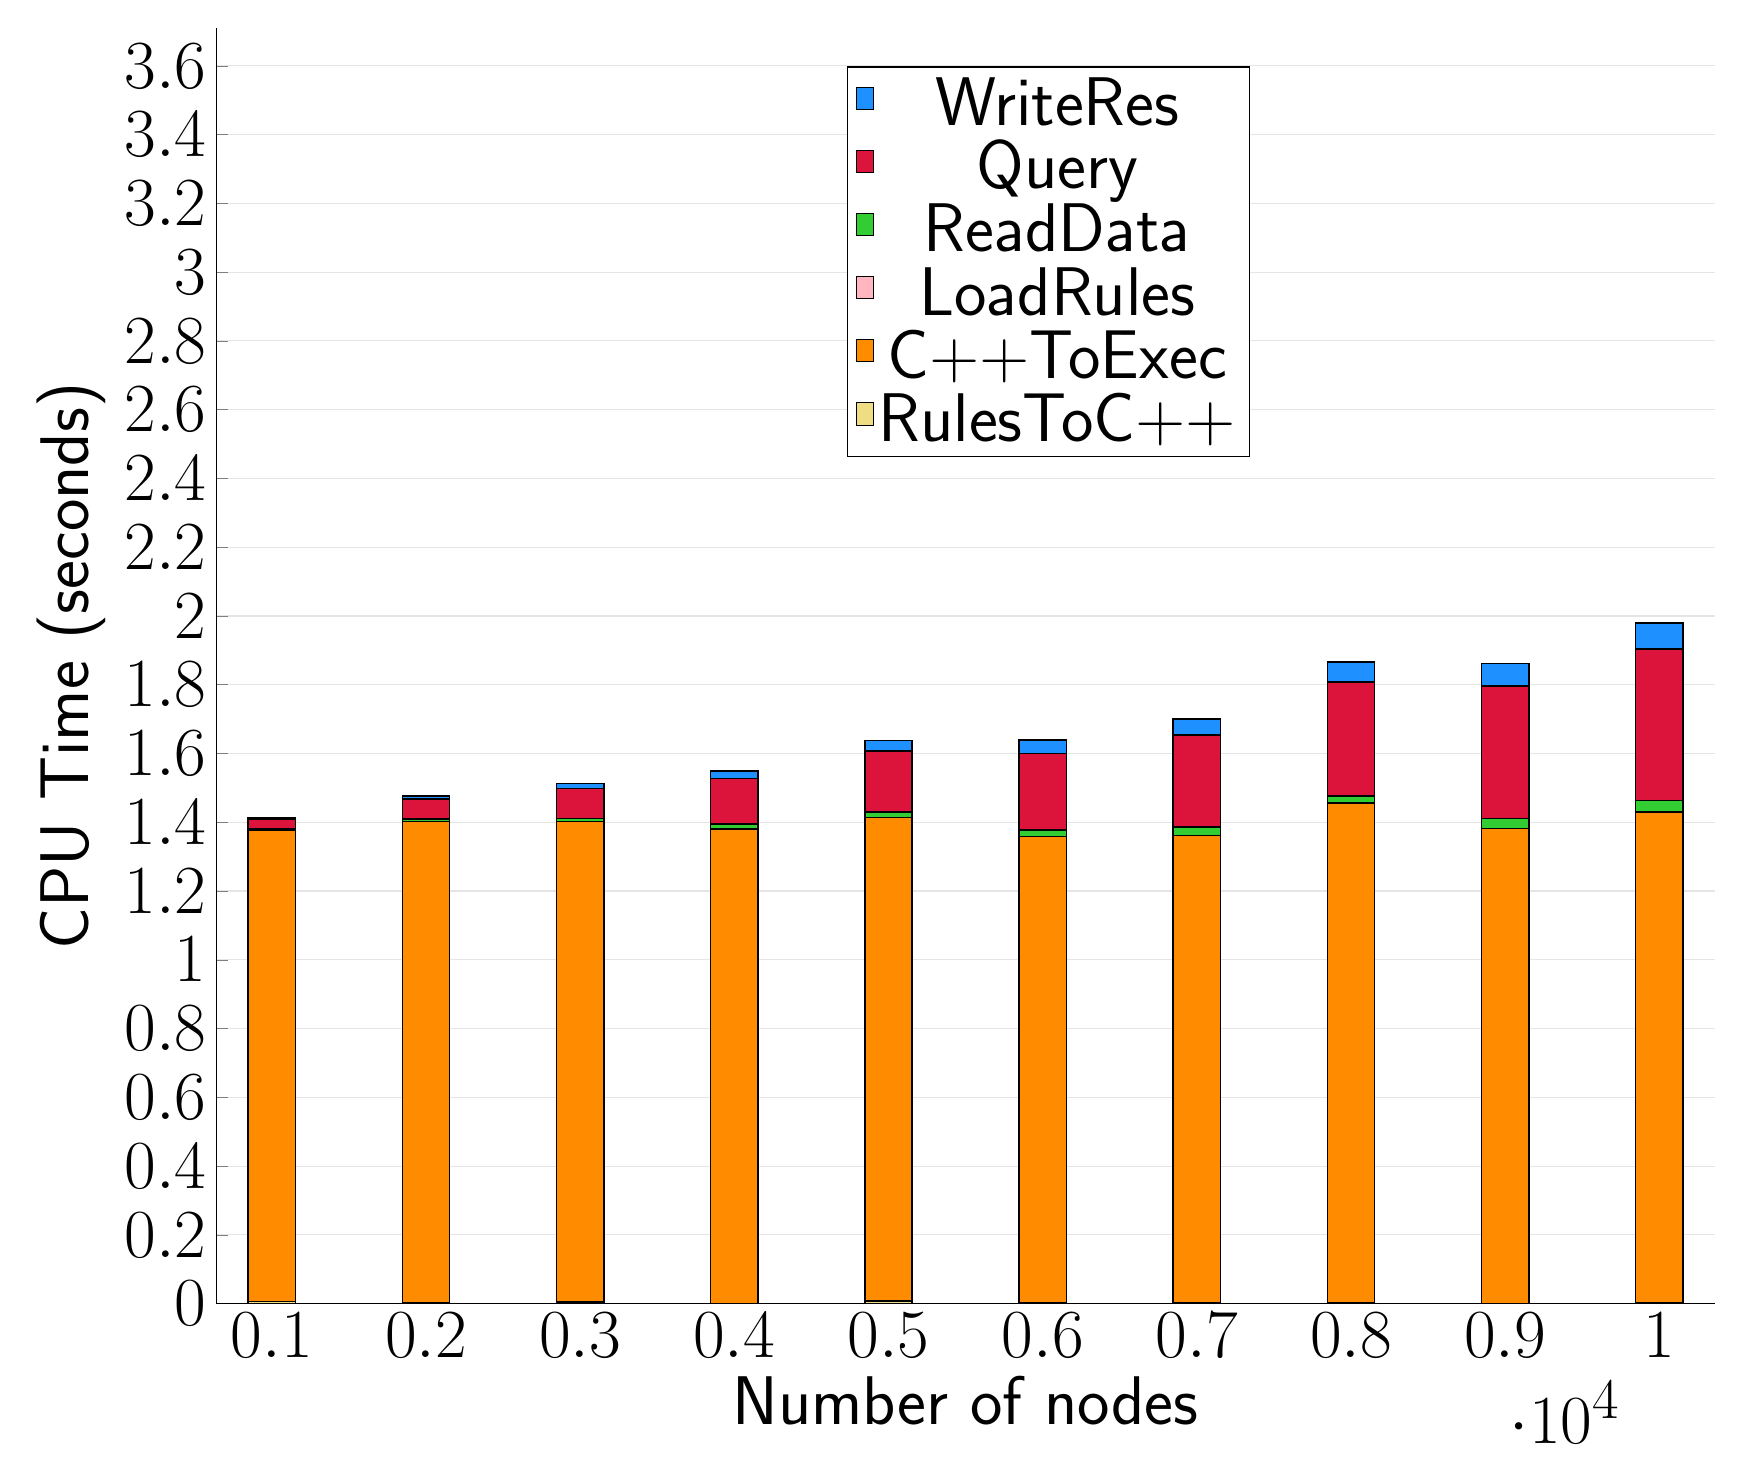
\begin{tikzpicture}
\begin{axis}[
   ybar stacked,
   width=1.7\textwidth,
   bar width=0.6cm,
   ymajorgrids, tick align=inside,
   major grid style={draw=gray!20},
   xtick=data,
   ymin=0, ymax=3.70944,
   axis x line*=bottom,
   axis y line*=left,
   enlarge x limits=0.04,
   legend style={
       at={(0.69, 0.97)},
       anchor=north east,
       legend columns=1,
       font=\Huge,
   },
   ylabel={CPU Time (seconds)},
   xlabel={Number of nodes},
   label style={font=\Huge},
   tick label style={font=\Huge},
]
\addlegendimage{fill=DodgerBlue, draw=black, line width=0.2pt}
\addlegendentry{WriteRes}
\addlegendimage{fill=Crimson, draw=black, line width=0.2pt}
\addlegendentry{Query}
\addlegendimage{fill=LimeGreen, draw=black, line width=0.2pt}
\addlegendentry{ReadData}
\addlegendimage{fill=LightPink, draw=black, line width=0.2pt}
\addlegendentry{LoadRules}
\addlegendimage{fill=DarkOrange, draw=black, line width=0.2pt}
\addlegendentry{C++ToExec}
\addlegendimage{fill=LightGoldenrod, draw=black, line width=0.2pt}
\addlegendentry{RulesToC++}
\addplot +[fill=LightGoldenrod, draw=black, line width=0.55pt] coordinates {
(1000, 0.006000000000000005)
(2000, 0.0020000000000000018)
(3000, 0.0040000000000000036)
(4000, 0.0)
(5000, 0.008000000000000007)
(6000, 0.0020000000000000018)
(7000, 0.0020000000000000018)
(8000, 0.001999999999999999)
(9000, 0.0)
(10000, 0.001999999999999999)
};
\addplot +[fill=DarkOrange, draw=black, line width=0.55pt] coordinates {
(1000, 1.372)
(2000, 1.4)
(3000, 1.3980000000000001)
(4000, 1.3800000000000001)
(5000, 1.4060000000000001)
(6000, 1.356)
(7000, 1.36)
(8000, 1.4540000000000002)
(9000, 1.3820000000000001)
(10000, 1.4279999999999997)
};
\addplot +[fill=LightPink, draw=black, line width=0.55pt] coordinates {
(1000, 0.0001446)
(2000, 0.000106)
(3000, 0.00011020000000000001)
(4000, 0.000164)
(5000, 0.0001566)
(6000, 0.0001364)
(7000, 0.000154)
(8000, 7.659999999999999e-05)
(9000, 0.0001562)
(10000, 0.0001566)
};
\addplot +[fill=LimeGreen, draw=black, line width=0.55pt] coordinates {
(1000, 0.0042452)
(2000, 0.007078999999999999)
(3000, 0.0089166)
(4000, 0.0153758)
(5000, 0.0163984)
(6000, 0.018841000000000004)
(7000, 0.023708)
(8000, 0.019599)
(9000, 0.029187)
(10000, 0.032827999999999996)
};
\addplot +[fill=Crimson, draw=black, line width=0.55pt] coordinates {
(1000, 0.027017400000000004)
(2000, 0.057820800000000006)
(3000, 0.0864642)
(4000, 0.1311474)
(5000, 0.1774304)
(6000, 0.22317820000000005)
(7000, 0.2681074)
(8000, 0.33294379999999996)
(9000, 0.3843542)
(10000, 0.44071319999999997)
};
\addplot +[fill=DodgerBlue, draw=black, line width=0.55pt] coordinates {
(1000, 0.0045406)
(2000, 0.0089114)
(3000, 0.015159200000000001)
(4000, 0.0221114)
(5000, 0.0299446)
(6000, 0.03872360000000001)
(7000, 0.0463576)
(8000, 0.057320399999999994)
(9000, 0.06545959999999999)
(10000, 0.0751884)
};
\end{axis}
\end{tikzpicture}

\end{document}
